In this section, we discuss the performance of \pred\ (\gt) against the other baselines in the latent bandit setting and create a generalized bilinear bandit setting. 
%
%
Note that the number of tasks $\Mpr \gg A \geq n$.
%
% Finally recall that when the horizon is small the weak demonstrator $\pi^w$ does not have sufficient samples for each action. This leads to a poor approximation of the greedy action. 
%
Using this experiment, we want to evaluate the ability of \pred\ (\gt) to exploit the underlying reward correlation when the horizon is small, the number of tasks is large, and understand its performance in the latent bandit setting \citep{hong2020latent, maillard2014latent, pal2023optimal, kveton2017stochastic}.
%
We create a latent bandit setting which generalizes the bilinear bandit setting \citep{jun2019bilinear, lu2021low, kang2022efficient, mukherjee2023multi}.
%
Again note that this setting also goes beyond the linear feedback model \citep{abbasi2011improved, lattimore2020bandit} and is related to matrix bandits \citep{yang2020reinforcement}.


\textbf{Latent bandit setting:} In this special multi-task latent bandits the learner is again provided with two sets of action sets, $\X\subseteq\R^{d_1}$ and $\Z\subseteq\R^{d_2}$ which are referred to as the left and right action sets. 
% At every round $t$ the learner chooses a pair of actions $\bx_t\in\X$ and $\bz_t\in\Z$ and observes a reward 
% \begin{align*}
%     r_t = \bx_t^\top \bTheta_* \bz_t + \eta_t
% \end{align*}
% where $\bTheta_*\in\R^{d_1\times d_2}$ is the unknown hidden matrix which is also low-rank. The $\eta_t$ is a $\sigma^2$ sub-Gaussian noise. 
% 
The reward for the $m$-th task at round $t$ is given by
\begin{align*}
    r_{m,t} = \bx_{m,t}^\top \underbrace{(\bTheta_{m,*} + \bU\bV^\top)}_{\bZ_{m_*}}\bz_{m,t} + \eta_{m,t}.
\end{align*}
Here  $\bTheta_{m,*}\in\R^{d_1\times d_2}$ is the unknown hidden matrix for each task $m$, which is also low-rank. 
%
Additionally, all the tasks share a \emph{common latent parameter matrix} $\bU\bV^\top \in \R^{d_1\times d_2}$ which is also low rank. Hence the learner needs to learn the latent parameter across the tasks hence the name latent bandits.
%
Finally, the $\eta_{m,t}$ is a $\sigma^2$ sub-Gaussian noise. Let $\kappa$ be the rank of each of these matrices $\bTheta_{m, *}$ and $\bU\bV^\top$.
%
Again special case is the rank $1$ structure where the reward for the $m$-th task at round $t$ is given by
\begin{align*}
    r_{m,t} = \bx_{m,t}^\top \underbrace{(\btheta_{m,*}\btheta_{m,*}^\top + \bu\bv^\top)}_{\bZ_{m, *}}\bx_{m,t} + \eta_{m,t}.
\end{align*}
%
where $\btheta_{m,*}\in\R^d$ for each task $m$ and $\bu, \bv\in\R^d$. Note that the left and right action sets are the same such that $\bx_{m,t} \in \X \subseteq \R^{d}$.

\textbf{Baselines:} We again implement the same baselines discussed in \Cref{sec:short-horizon}. The baselines are \pred, \predt, \dptg, \ad, \ts, and \estr. However, we now implement a special \estr\ (stated in \Cref{sec:bilinear}) which has knowledge of the shared latent parameters $\bU$, and $\bV$. We call this the \estro\ algorithm. Therefore \estro\ has knowledge of the problem parameters in the latent bandit setting and hence the name. 
%
Again note that we do not implement the \linucb\ and \mlin\ for the latent bandit setting.
%



\textbf{Outcomes:} We first discuss the main outcomes of our experimental results for increasing the horizon:

\begin{tcolorbox}
\customfinding \pred\ (\gt) outperforms \dptg, \ad, and matches the performance of \estro\ in latent bandit setting. 
\end{tcolorbox}

% \noindent
% \textbf{(1)} The \pred\ (\gt) learns to exploit the underlying latent bilinear structure and reward correlation between the different tasks even when $A \geq n$ but $\Mpr \gg A$.

% \textbf{(2)} The \pred\ (\gt) has lower regret than its weak demonstrator \ts\ which does not know the underlying latent structure.  The \pred\ (\gt) has lower regret compared to \dptg.

% \textbf{(3)} The \pred\ (\gt) has regret that is closer to \estro.

% \begin{figure}[!hbt]
% \centering
% \begin{tabular}{ccc}
% %%%%%%%%%%
% \hspace*{-1.5em}\subfigure[Rank $1$ $\bZ_{m,*}$]{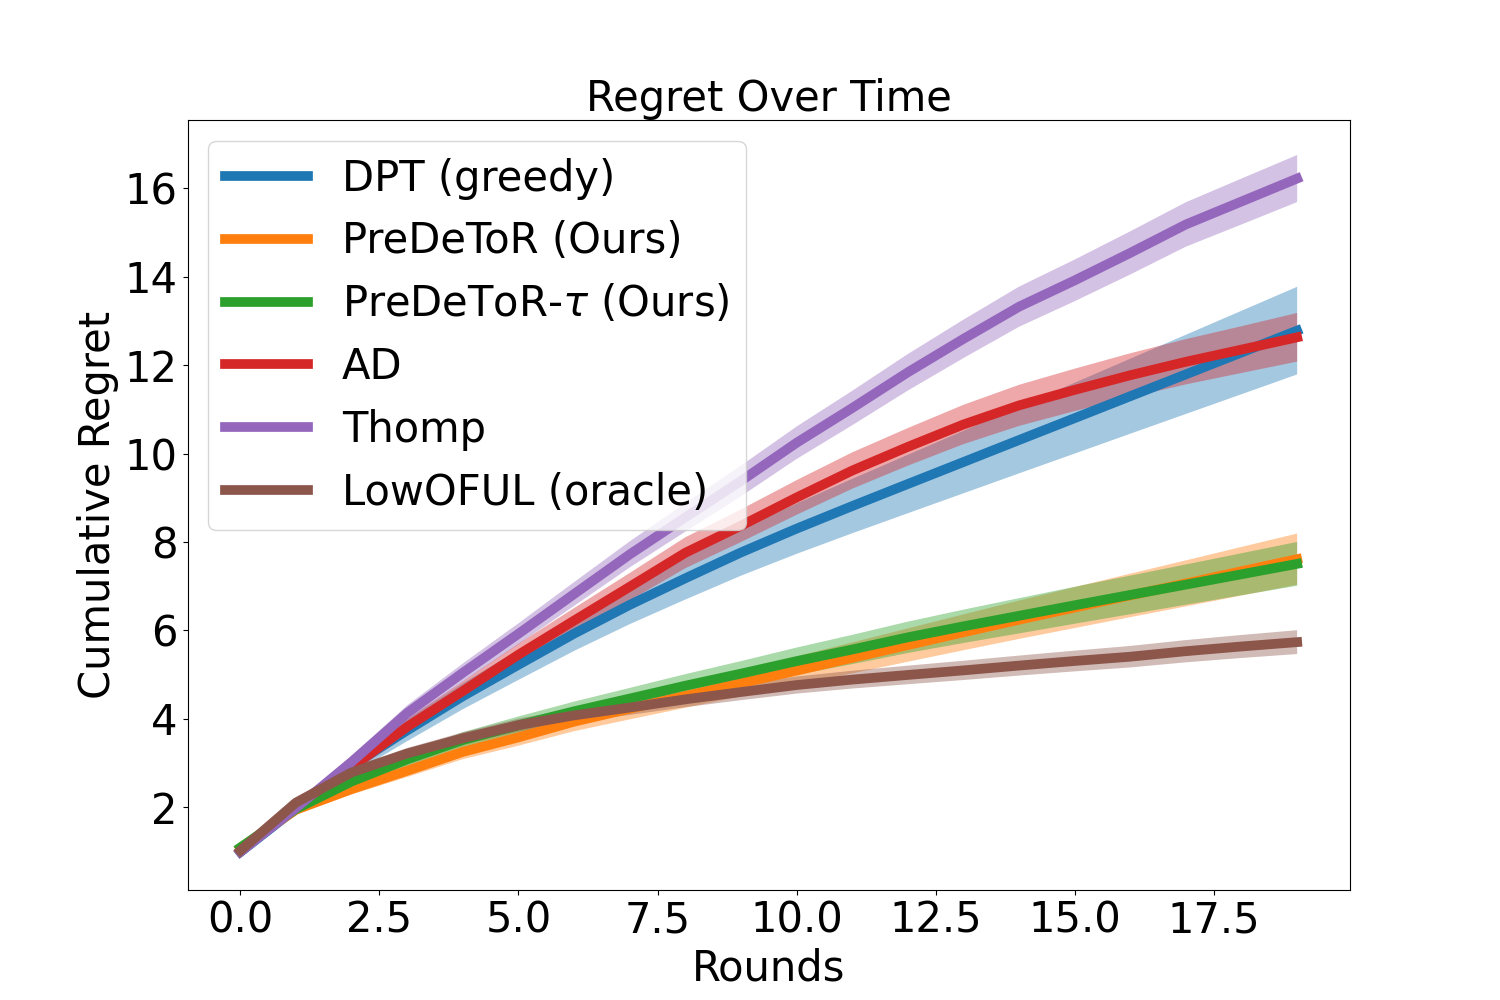
\includegraphics[scale = 0.13]{img/Neurips/latent/lat_1_lr0.00015_do0_embd32_layer4_head4_envs250080_hists1_samples1_var0.3_cov0.0_H20_d20_lind3_seed1_testcov0.0_hor20.pkl.png} \label{fig:latent-1}} &
% %%%%%%%%%%%%%%%%%%%%%%%%%%%%%%%
% \hspace*{-1.5em}\subfigure[Rank $2$ $\bZ_{m,*}$]{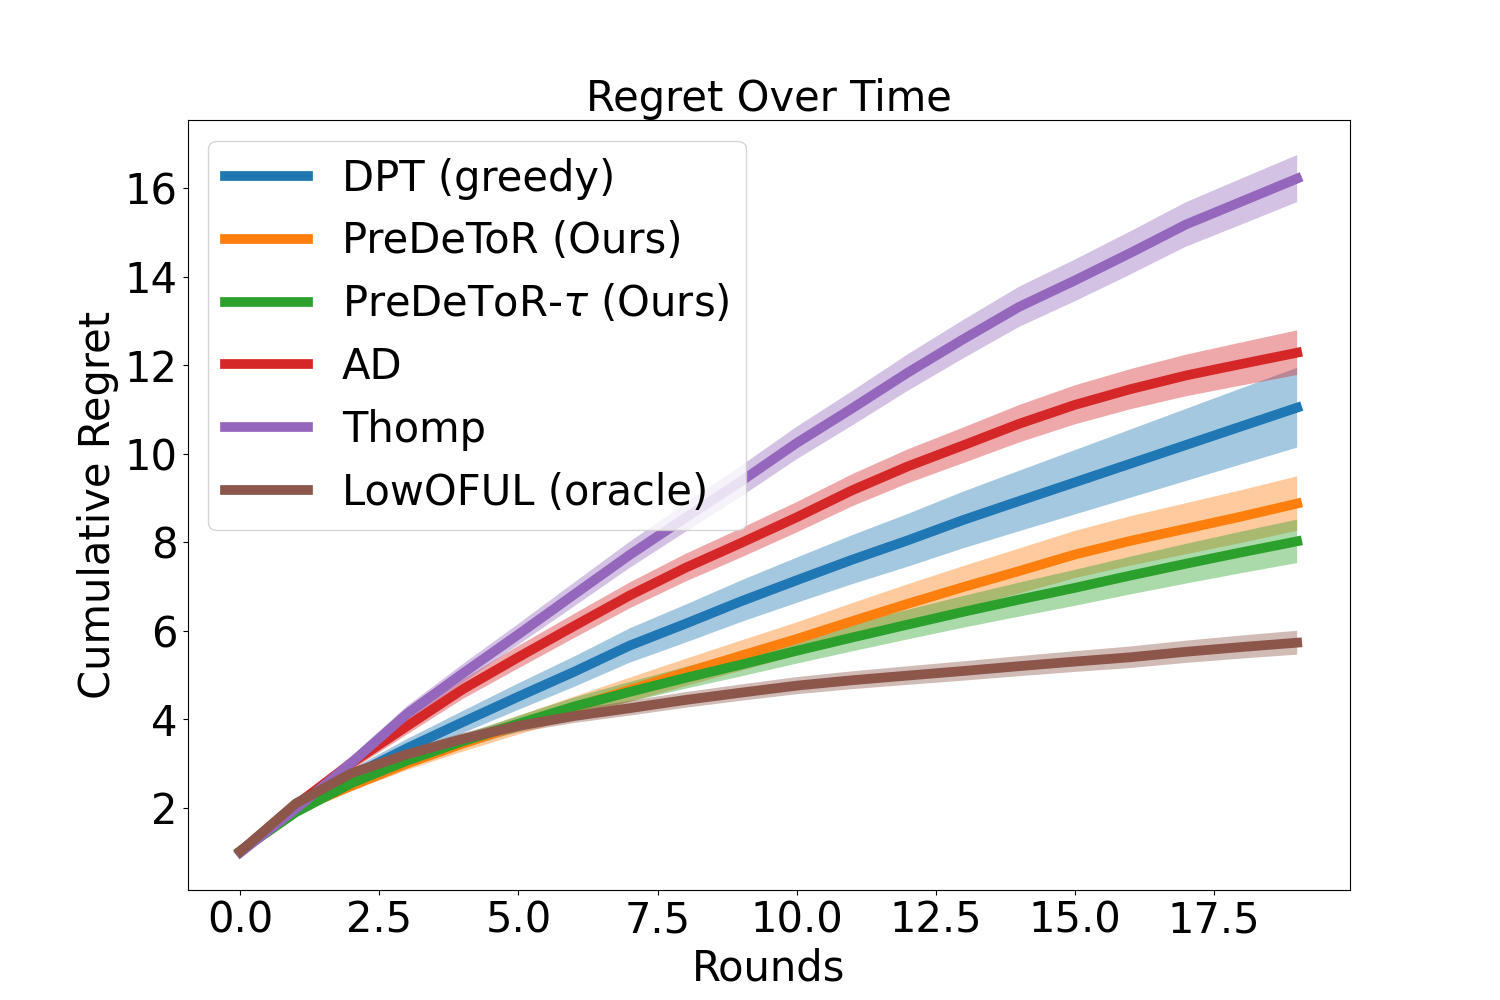
\includegraphics[scale = 0.13]{img/Neurips/latent/lat_2_lr0.00015_do0_embd32_layer4_head4_envs250050_hists1_samples1_var0.3_cov0.0_H20_d20_lind3_seed1_testcov0.0_hor20.pkl.png} \label{fig:latent-2}}
% %%%%%%%%%%%%%%%%%%%%%%%%%%%%%%
% \hspace*{-1.5em}\subfigure[Rank $3$ $\bZ_{m,*}$]{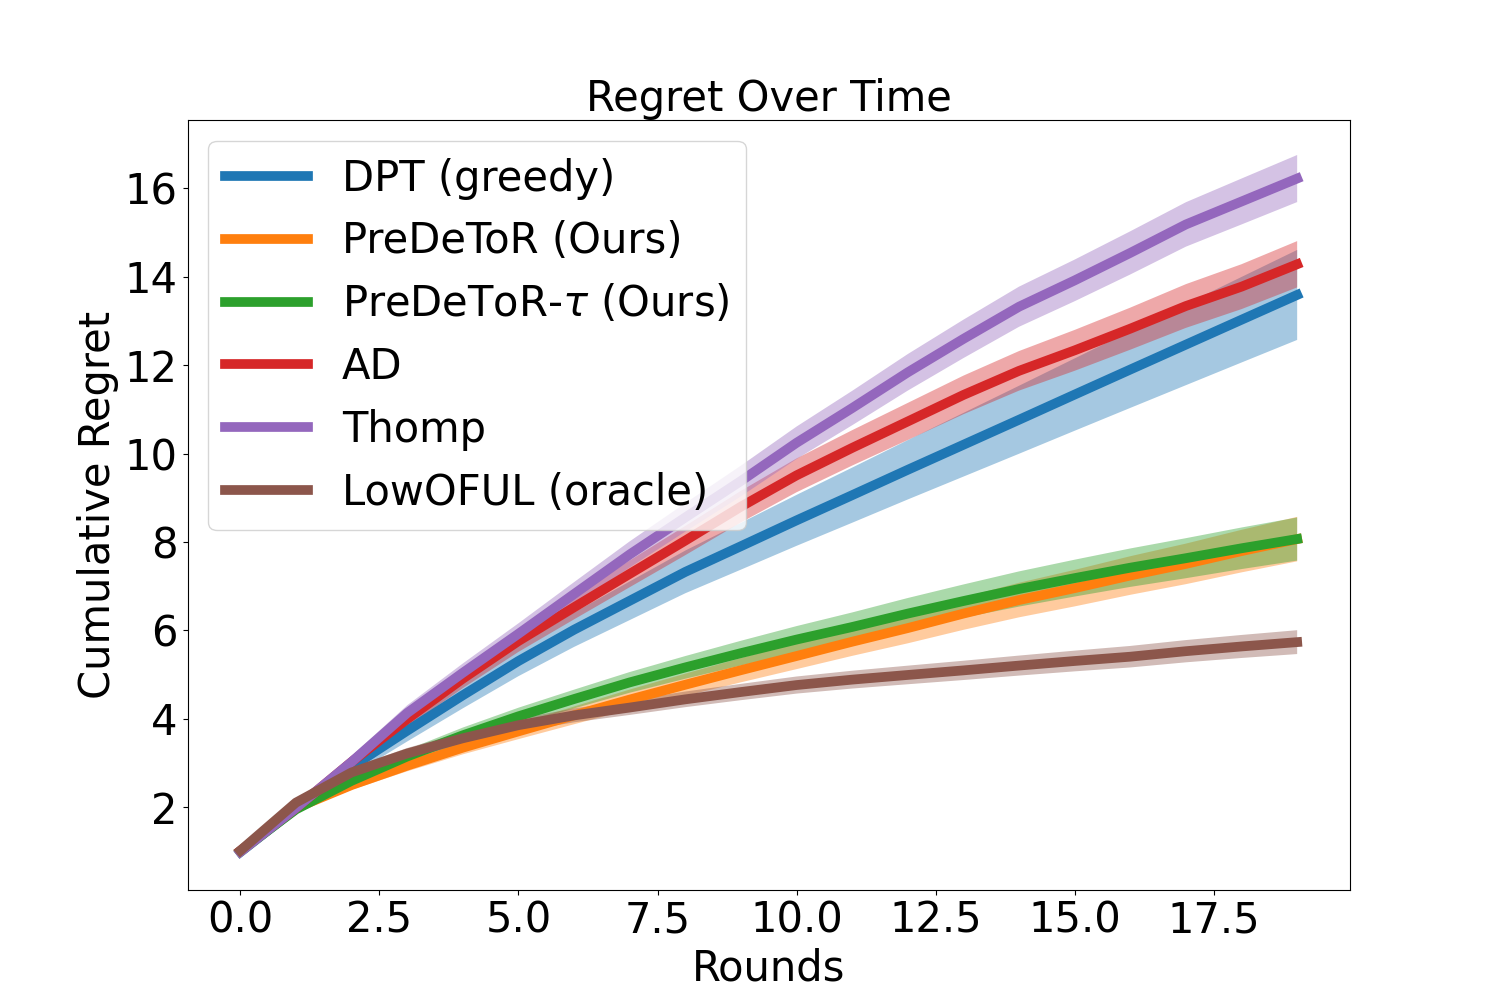
\includegraphics[scale = 0.13]{img/Neurips/latent/lat_3_lr0.00015_do0_embd32_layer4_head4_envs200950_hists1_samples1_var0.3_cov0.0_H20_d20_lind3_seed1_testcov0.0_hor20.pkl.png} \label{fig:latent-3}}
% \end{tabular}
% \vspace*{-1em}
% \caption{Experiment with latent bandits. The y-axis shows the cumulative regret.}
% \label{fig:expt-latent}
% \end{figure}

\begin{figure}[!hbt]
\centering
\begin{subfigure}[b]{0.32\textwidth}
   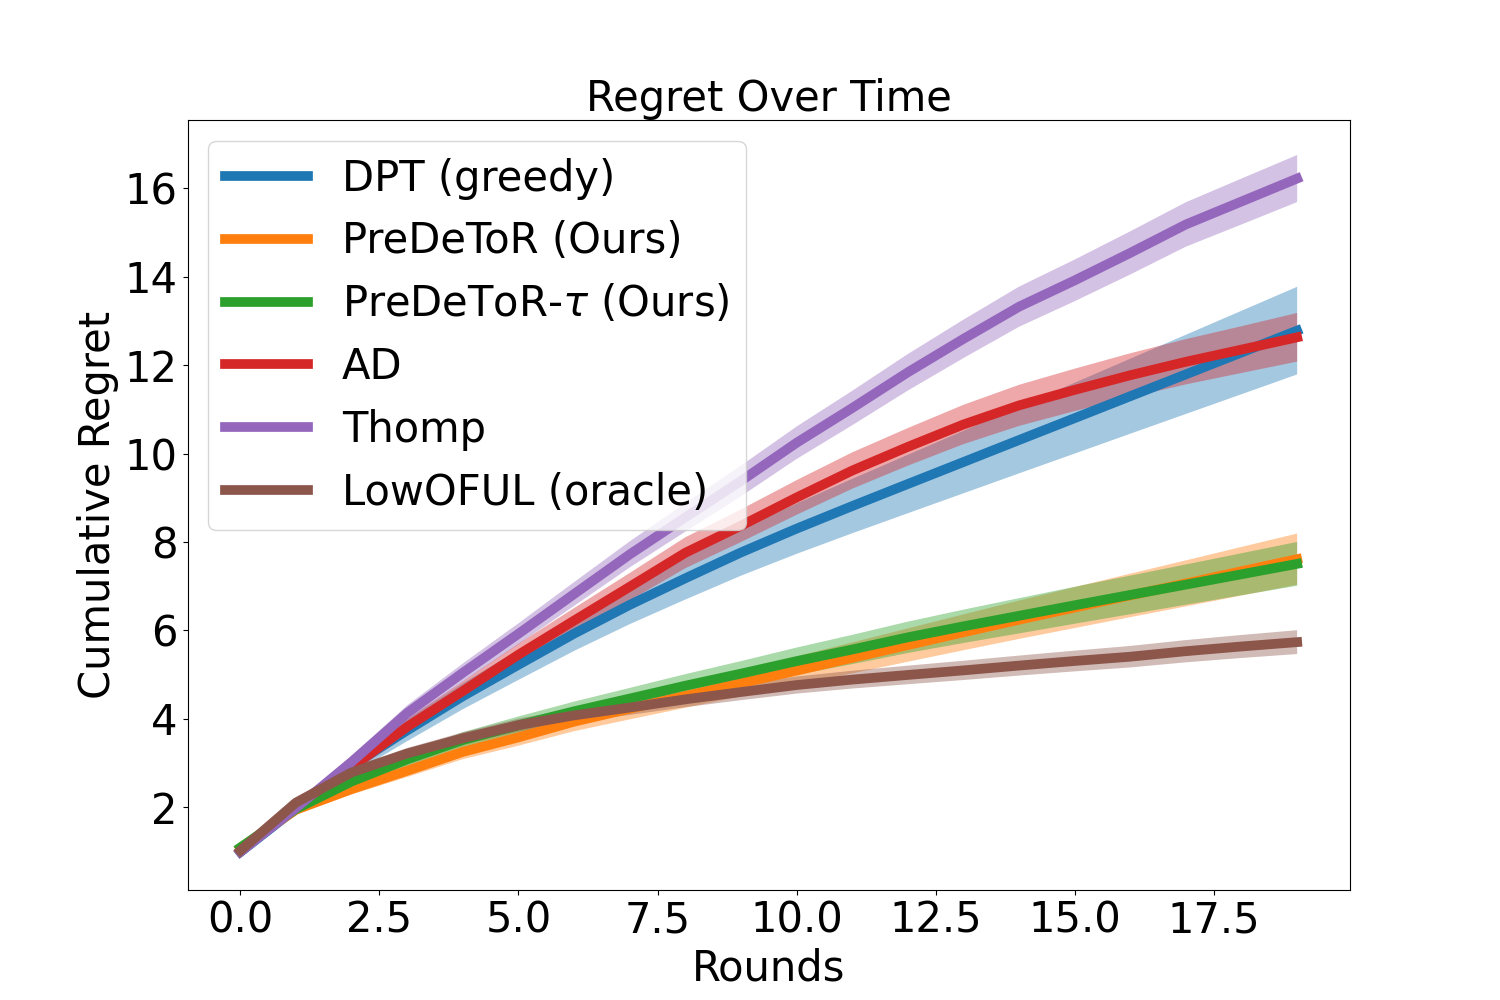
\includegraphics[scale=0.13]{img/Neurips/latent/lat_1_lr0.00015_do0_embd32_layer4_head4_envs250080_hists1_samples1_var0.3_cov0.0_H20_d20_lind3_seed1_testcov0.0_hor20.pkl.png}
   \caption{Rank $1$ $\bZ_{m,*}$}
   \label{fig:latent-1}
\end{subfigure}%
\begin{subfigure}[b]{0.32\textwidth}
   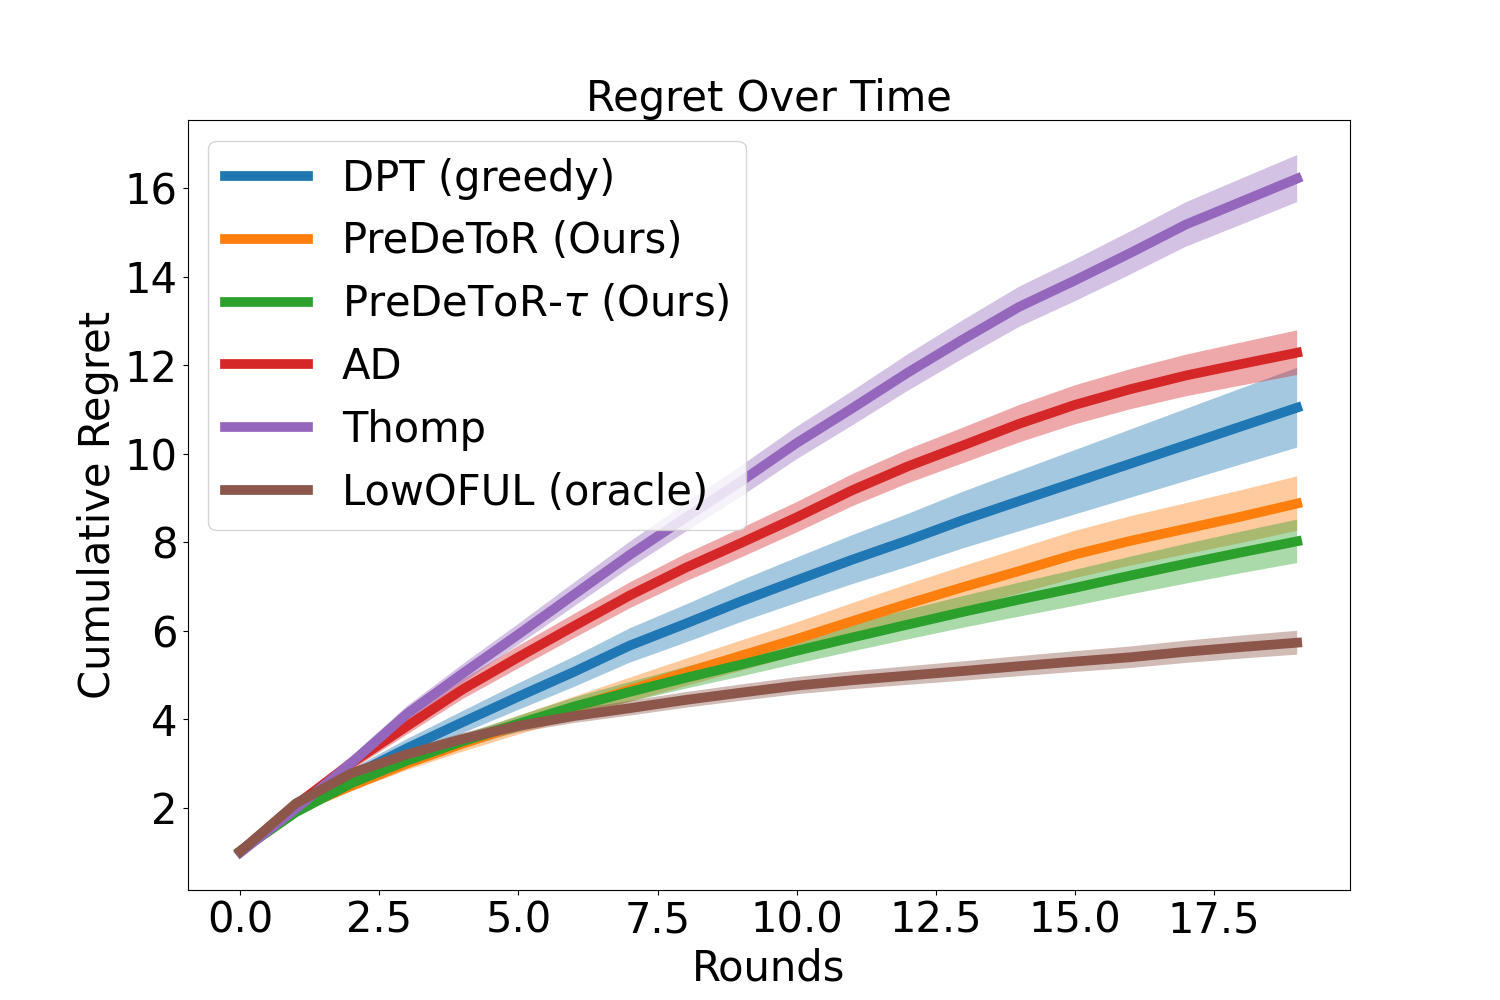
\includegraphics[scale=0.13]{img/Neurips/latent/lat_2_lr0.00015_do0_embd32_layer4_head4_envs250050_hists1_samples1_var0.3_cov0.0_H20_d20_lind3_seed1_testcov0.0_hor20.pkl.png}
   \caption{Rank $2$ $\bZ_{m,*}$}
   \label{fig:latent-2}
\end{subfigure}%
\begin{subfigure}[b]{0.32\textwidth}
   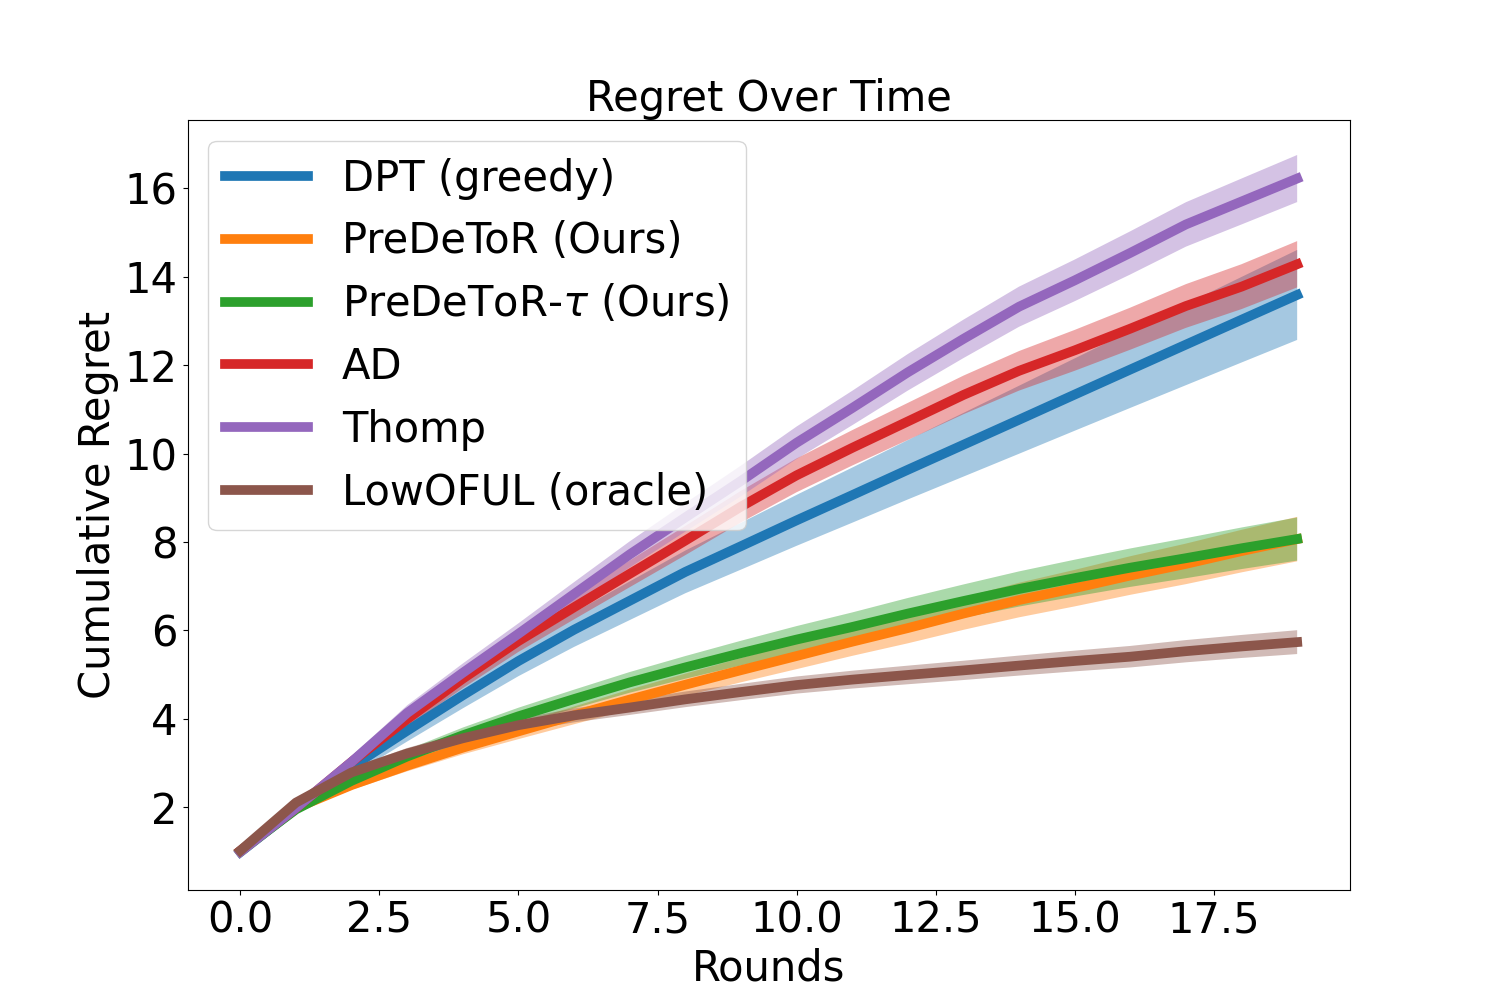
\includegraphics[scale=0.13]{img/Neurips/latent/lat_3_lr0.00015_do0_embd32_layer4_head4_envs200950_hists1_samples1_var0.3_cov0.0_H20_d20_lind3_seed1_testcov0.0_hor20.pkl.png}
   \caption{Rank $3$ $\bZ_{m,*}$}
   \label{fig:latent-3}
\end{subfigure}
\vspace*{-1em}
\caption{Experiment with latent bandits. The y-axis shows the cumulative regret.}
\label{fig:expt-latent}
\end{figure}


\textbf{Experimental Result:} We observe these outcomes in \Cref{fig:expt-latent}. In \Cref{fig:latent-1} we experiment with rank $1$ hidden parameter $\btheta_{m,*}\btheta_{m,*}^\top$ and latent parameters $\bu\bv^\top$ shared across the tasks and set horizon $n=20$, $\Mpr =  200000$, $\Mts = 200$, $A=30$, and $d=5$. 
%
In \Cref{fig:latent-2} we experiment with rank $2$ hidden parameter $\bTheta_{m,*}$, and latent parameters $\bU\bV^\top$ and set horizon $n=20$, $\Mpr =  250000$, $\Mts = 200$, $A=25$, and $d=5$. 
%
In \Cref{fig:latent-3} we experiment with rank $3$ hidden parameter $\bTheta_{m,*}$, and latent parameters $\bU\bV^\top$ and set horizon $n=20$, $\Mpr =  300000$, $\Mts = 200$, $A=25$, and $d=5$. 
%
Again, the demonstrator $\pi^w$ is the \ts\ algorithm. We observe that \pred\ (\gt) has lower cumulative regret than \dptg, \ad\ and \ts. Note that for any task $m$ for the horizon $20$ the \ts\ will be able to sample all the actions at most once.
% Moreover \pred\ matches the performance of \linucb. 
%
%The weak performance of \dptg\ can be attributed to both short horizons and the inability to estimate the optimal action for such a short horizon $H < A$. 
%
Note that for this small horizon setting the \dptg\ does not have a good estimation of $\widehat{a}_{m,*}$ which results in a poor prediction of optimal action $\widehat{a}_{m,t,*}$. In contrast \pred\ (\gt) learns the correlation of rewards across tasks and is able to perform well.
% This results in higher regret. 
Observe from \Cref{fig:latent-1}, \ref{fig:latent-2}, and \ref{fig:latent-3} that \pred\ has lower regret than \ts\ and has regret closer to \estro which has access to the problem-dependent parameters.
%
Hence. \estro\ outperforms \pred\ (\gt) in this setting.
%
% The training of \ad\ ensures that it does not outperform the demonstrator \ts.
%
% Also, this short horizon is not enough for \estr\ to learn the underlying $\bTheta_{m, *}$ with high precision. Hence, \pred\ also slightly lower regret than \estr. 
This shows that \pred\ is able to exploit the underlying latent structure and reward correlation better than \dptg, and \ad.
